از آنجایی که تسک پروژه NER بوده خیلی از مراحل این پروژه نتیجه مورد نظر را به ما نداد ولی سعی کردیم با مطالعه بر روی تجریبات بقیه، نتیجه ای که انتظار داشتیم را ذکر کنیم.

\huge
\LARGE{بخش word2vec}\\
\large
شباهت کسینوسی بین
vector word
های برچسب های
PERSON و LOC
را محاسبه کردیم و نتیجه به صورت زیر بوده است:
\begin{figure}[H]
    \centering
    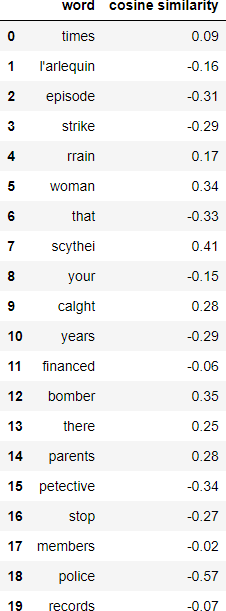
\includegraphics[width=0.4\linewidth]{../reports/word2vec_cosine_similarity.png}
   \end{figure}
   
همانطور که قابل مشاهده است: 
کلمات متدوالی مانند 
through
که در جملاتی که به مکان یا فرد خاصی اشاره میکنند به کار میروند، بردار وکتور هایشان شباهت بالایی دارد.
اما برای کلمه ای مثل l'arlequin
که اسم مکان است، میزان شباهت منفی است.

البته در کل صورت سوال احتمالا میخواست کاربردی بودن واژه ها در context های مختلف رو بررسی کند.
که با تسک NER ممکن نبود.
برای مثال بردار وکتور کلمه ی arrested
در داستان های دو ژانر جنایی و معمایی شباهت بیشتری دارند تا داستان های دو ژانر جنایی و /فانتزی
.

\huge
\LARGE{بخش language model}
\large

ابتدا مدل را روی کل داده ها FineTune میکنیم.
حجم مدل خیلی بزرگ میشود (3.1 گیگ)
خروجی تقریبا با محیط داستان ارتباط دارد.

\grayLBox{
0-  ive got what you need to prove sake's guilt in chow's case. 
\\
1-  ive got the upper hand this time. i can't believe i made this deal. 
\\
3-  ive got the lead on this one. ive got the upper hand this time, as always.
\\
4-  ive got everything i need to prove sake's guilt in chow's case. 
\\
5-  llyod and flemmings are locked and can't they see the purple hyacinth.
\\
6-  ive got some experience with hunting. i'm hunting down double agents
}

برای هر برچسب هم جدا آموزش دادیم.
اما دوباره مثل تسک قبل نتیجه دلخواه را نگرفتیم.
چون متونی که شامل یک برچسب میشوند context یکسانی ندارند 
و نمیشود از مدل توقع داشت در اون context برایمان متن تولید کند.
ولی میتوان انتظار داشت از واژه های مرتبط به آن برچسب استفاده کند.

 \textbf{برچسب PERSON}
 \\
 \\
 \grayLBox{
1-  I didn't send my personal messenger lieutenant hawkes over there just to ask someone to help me.\\
2-  dakan is home alone right now.\\
3-  Belladonna davenport Did you manage to get hand on the black swan?\\
4-   Hi, officer sinclair. }
\\
\\
اسم شخصیت های داستان در متن های تولید شده مشاهده میشود.
مثل:
\\
\lr{hawkes, dakan, belladonna davenport, officer sinclair}
\\
 \textbf{برچسب LOC}
 \\
 \\
\grayLBox{
1- ized recently learned about anslow's arrest. \\
2- ibrightened before the allendale bombing But \\
3- izhar chief is hent even ten years old. \\
4- ica talking about the allendale incident this morning
}
\\
\\
همانطور که مشاهده میکنیم، کلمه ی آلندل را بسیار به کار برده. 
حادثه قطار آلندل حادثه مهمی در داستان هست و اسم این مکان ها در طول داستان بار ها تکرار شده است.

\newpage
\huge
\LARGE{بخش augmentation data}\\
\large
در این قسمت به کمک 
\lr{chatgpt3.5}
دیتای آموزشی جدید تولید میکنیم.
prompt
استفاده شده:
\\
\\
\grayLBox{Generate a dataset for my NER model which contains LOC and PERSON entities.
                        The format should consist two elements: the first element is the text string, and the second element is a list of label annotations. Each label annotation is represented as a list containing three elements: the start index of the labeled entity the text, the end index of the labeled entity, and the label itself. the dataset must have list of arrays.
                        don't give any explainations.}
                        \\
                  

نمونه دیتای آموزشی تهیه شده از وبتون ها به صورت زیر بوده است:
\\
\\
\grayLBox{[
 ["you'd better not forget about anslow's picture . Sandman", [[51, 58, "PERSON"], [31, 37, "PERSON"]]],\newline
 ["only to be killed for it hundreds of people were killed for it i almost was too Mhk and dylan Sandman za It", [[94, 101, "PERSON"], [88, 93, "PERSON"]]],\newline
 ["was it was a lie No sandman knew him His body missing . There", [[20, 27, "PERSON"]]]
]}
\newpage
داده تولید شده توسط
\lr{chatgpt3.5}
:
\\
\\
\grayLBox{
[
  ["John Smith went to Paris for vacation.", [[0, 10, "PERSON"], [18, 23, "LOC"]]], \newline
  ["London is a beautiful city.", [[0, 6, "LOC"]]],
  ["Mary visited the Eiffel Tower in Paris.", [[0, 4, "PERSON"], [24, 29, "LOC"]]],\newline
  ["New York City is known for its skyscrapers.", [[0, 14, "LOC"]]],\newline
  ["Michael Jordan played basketball for the Chicago Bulls.", [[0, 14, "PERSON"], [31, 45, "LOC"]]]
]
}



\huge
\LARGE{انجام NER توسط OpenAI}\\
\large
prompt
استفاده شده:
\\
\\
\grayLBox{Find Location and Person entities in this text, just tell which words are the entities, not further explanation needed:\newline At the Carmine Camelia, Kieran and Lauren end up being locked up in a supply closet after. To avoid drawing attention, they decide to wait until closing time to kick the door open.
Lauren realizes that the failure in their spying devices happened because they both used the same type of technology, and the signals interfered with one another. She is uncomfortable by the whole situation and tells Kieran to stay away from her then sits further from him.}
                        \\

                  
   
لینک \lr{github} :

 \begin{latin}
 \url{https://github.com/Bayany/NLP_NER}
 \end{latin}

لینک \lr{huggingface}:
 \begin{latin}
\url{https://huggingface.co/datasets/Bayany/NER}
 \end{latin}
 
